\documentclass[crop,tikz]{standalone}
\usetikzlibrary{positioning,arrows,fit,calc,shapes.symbols,shapes.geometric}
\pgfdeclarelayer{bg}
\pgfsetlayers{bg,main}
\tikzset{
	>=stealth'
}
\makeatletter
\pgfdeclareshape{document}{
	\inheritsavedanchors[from=rectangle] % this is nearly a rectangle
	\inheritanchorborder[from=rectangle]
	\inheritanchor[from=rectangle]{center}
	\inheritanchor[from=rectangle]{north}
	\inheritanchor[from=rectangle]{south}
	\inheritanchor[from=rectangle]{west}
	\inheritanchor[from=rectangle]{east}
	% ... and possibly more
	\backgroundpath{% this is new
		% store lower right in xa/ya and upper right in xb/yb
		\southwest \pgf@xa=\pgf@x \pgf@ya=\pgf@y
		\northeast \pgf@xb=\pgf@x \pgf@yb=\pgf@y
		% compute corner of ‘‘flipped page’’
		\pgf@xc=\pgf@xb \advance\pgf@xc by-7.5pt % this should be a parameter
		\pgf@yc=\pgf@yb \advance\pgf@yc by-7.5pt
		% construct main path
		\pgfpathmoveto{\pgfpoint{\pgf@xa}{\pgf@ya}}
		\pgfpathlineto{\pgfpoint{\pgf@xa}{\pgf@yb}}
		\pgfpathlineto{\pgfpoint{\pgf@xc}{\pgf@yb}}
		\pgfpathlineto{\pgfpoint{\pgf@xb}{\pgf@yc}}
		\pgfpathlineto{\pgfpoint{\pgf@xb}{\pgf@ya}}
		\pgfpathclose
		% add little corner
		\pgfpathmoveto{\pgfpoint{\pgf@xc}{\pgf@yb}}
		\pgfpathlineto{\pgfpoint{\pgf@xc}{\pgf@yc}}
		\pgfpathlineto{\pgfpoint{\pgf@xb}{\pgf@yc}}
		\pgfpathlineto{\pgfpoint{\pgf@xc}{\pgf@yc}}
	}
}
\makeatother

\begin{document}
	
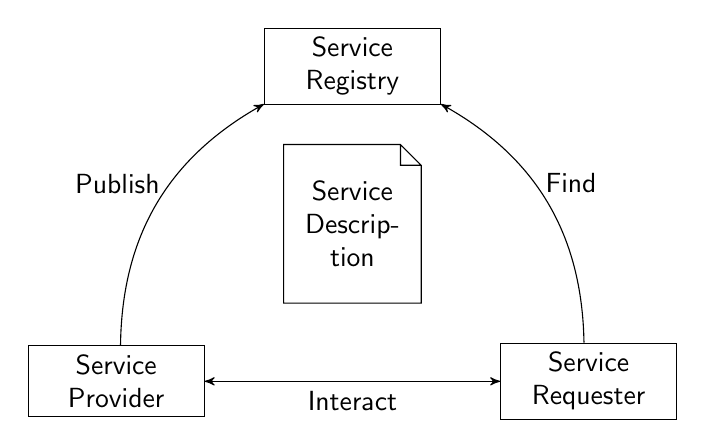
\begin{tikzpicture}[
node distance = 20mm,
every node/.style = {
	font = \sffamily
},
script/.style = {
	shape=document,
	draw,
	%line width=1pt,
	text width=1.5cm,
	minimum height=2cm,
	align=center
},
component/.style = {
	draw,
	text width = 2cm,
	align = center
}
]
	
\node[script] (decr) at (0,0) {Service Description};
\node[component] (reg) at (0,2) {Service Registry};
\node[component] (prov) at (-3,-2) {Service Provider};
\node[component] (req) at (3,-2) {Service Requester};

\draw[bend left,->] (prov) to node[above,xshift=-5mm] {Publish} (reg);
\draw[bend right,->] (req) to node[above,xshift=3mm] {Find} (reg);
\draw[<->] (prov) -- node[below] {Interact} (req);
	
\end{tikzpicture}

\end{document}